%!TEX root = ../main.tex
\subsubsection{Metric spaces and convergences}

In this part we will see how the tools we developed can be deployed in practice. First we extend the notion of Lebesgue integrability by using the concept of almost everywhere. The we see how handle different kind of limits of series of functions.

\paragraph{The space $L^1$} As we discovered that many properties can be useful even when they holds almost everywhere, now we can find a space wider than $\Lc_1$ but whose functions has the same properties.

\begin{defn}\label{L1-space}
	Consider the space $\Lc_1(\Omega, \mm, \mu)$ and define on it the following equivalence relation: 
	$$
		f \sim g 
		\quad \text{ if }  
		f = g 
		\text{ a.e. in }\Omega
	;
	$$
	we define the \emph{space $L_1$} by the quotient set:
	$$L_1(\Omega, \mm, \mu)=\frac{\Lc_1(\Omega, \mm, \mu)}{\sim}.$$
\end{defn}

In plain language, this set contains all the functions which are equal almost everywhere to a function in $\Lc^1$.
For the definition of quotient set see \vref{defn-equiv-class-quot-set}.

Such set is a vector space on $\RR$ with respect to the canonical operations sum $[f]+[g]=[f+g]$ and homogeneity $[c f] = c[f]$, $c \in \RR$.\\
It is also a metric space with respect to the following distance:
$$
	d_1 
	\coloneqq \int_\Omega |f-g| \, \de \mu
	\text{ for all } [f],[g]
	\in L_1(\Omega, \mm, \mu)
,
$$
and is proved that $L^1$ with $d_1$ is a complete metric space.\\
However, $\Lc_1$ isn't a metric space with respect to the distance $d_1$ as $d_1(f,g) = 0$ implies only that $f=g$ a.e. in $\Omega$.

As $L^1$ is a metric space we can develop a proper notion of convergence on it.

\paragraph{Convergence of series of functions} There are four notions of convergence in a measure space: we will introduce the definition and we analyze the relations between them.
\begin{defn}
	Let $(\Omega, \mm, \mu)$ be a complete measure space, and $\{f_n\}_{n\in \NN}$ be a sequence of measurable functions such that $f_n : \Omega \to \RR$:
	\begin{itemize}
		\item we say that $f_n(t)$ \emph{converges point-wise almost everywhere} to $f(t)$ as $n\to \infty$,
			and we write ``$f(t)_n \aeto f(t)$'',
			if we have:
			$$
				\mu (\{t \in \Omega: \lim\limits_{n \to +\infty} f_n(t) \neq f(t)\})
				= 0
			;
			$$
			
		\item we say that $f_n(t)$ \emph{converges uniformly almost everywhere} to $f(t)$ as $n\to \infty$,
			and we write ``$f(t)_n \uaeto f(t)$'',
			if we have:
			$$
				\lim\limits_{n \to +\infty}\underset{\Omega}{\esssup} |f_n-f| 
				= 0
			;
			$$
			
		\item we say that $f_n(t)$ \emph{converges in mean} to $f(t)$ as $n\to \infty$,
			and we write ``$f(t)_n \lto{1} f(t)$'',
			if $\{f_n\}_{n \in\NN} \subset L^1(\Omega, \mm, \mu)$ and: 
			$$
				\lim\limits_{n \to +\infty} \int_\Omega |f_n-f| \,\de \mu 
				= 0
			;
			$$
			
		\item we say that $f_n(t)$ \emph{converges in measure} to $f(t)$ as $n\to \infty$,
			and we write ``$f(t)_n \mto f(t)$'',
			if we have:
			$$
				\forall \varepsilon >0 
				\quad \lim\limits_{n \to +\infty} \mu(\{t\in \Omega : |f_n (t)-f(t)| > \varepsilon \}) 
				= 0
			.
			$$
	\end{itemize}
\end{defn}
To memorize those definition notice that there are some elements that are common; the following observations can help to understand and memorize:
\begin{itemize}
	\item the $\lim_{n \to \infty}$ occurs in all definitions;
	\item all definitions states that some quantity is equal to zero;
	\item all definitions involves the set $\Omega$;
	\item all definitions involves the measure $\mu$, the first and the second through a measure of a set, the third through the integral, and the second through the $\esssup$, which is defined in accordance to a measure.
	\item all definitions involves $f_n - f$, which, in different ways, tends to zero. Also the first contains this subtraction implicitly;
	\item notice that the third definition requires also that the functions are integrable a.e.;
	\item the first definition consist of a measure of the set in which a limit does not occur, viceversa the third is the limit of the measure of a set.
\end{itemize}

It's clear that this definitions are not fully equivalent each other, but they are somehow correlated. Here we try to investigate their relations by declaring and proving some propositions.

Some observation before starting the comparisons. Notice that the main vantage of uniform convergence over point-wise is that with uniform convergence we have not any dependence form the points of the domain $t$.\\ 
Notice that the integral in the mean convergence contains the distance $d_1$ (the module): that is a metric convergence.\\
The convergence in measure is widely used in probability.

\paragraph{Uniform a.e.\ convergence implies point-wise a.e.\ convergence} This result is stated in the following proposition:
\begin{prop}\label{convergence-uniform-implies-point-wise}
	If a series of function converges uniformly almost everywhere, then such series also converges point-wise almost everywhere.
\end{prop}
The proof is very easy. Do it!\\

\paragraph{Point-wise a.e.\ convergence does NOT imply uniform a.e.\ convergence} Consider the following series of functions:
$$f_n(t) = \begin{cases}
nt & \text{if }0 \leq t \leq \frac 1 n \\
2-nt & \text{if }\frac 1 n \leq t \leq \frac 2 n \\
0 & \text{if }\frac 2 n \leq t \leq 1
\end{cases}$$

\begin{figure}[htpb]
	\centering
	\tikzset{every picture/.style={line width=0.75pt}} %set default line width to 0.75pt        

	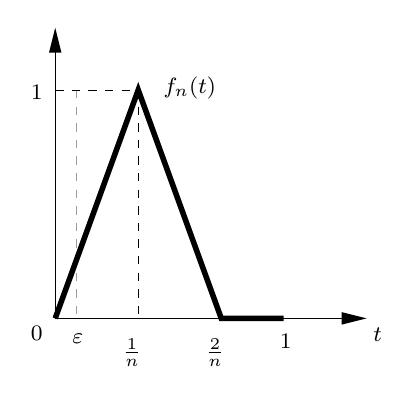
\begin{tikzpicture}[x=0.75pt,y=0.75pt,yscale=-1,xscale=1]
	%uncomment if require: \path (0,257); %set diagram left start at 0, and has height of 257

	\draw [color={rgb, 255:red, 155; green, 155; blue, 155 }  ,draw opacity=1 ] [dashed, very thin]  (230,60) -- (230,170);
	\draw (220,170) -- (368,170);
	\draw [shift={(370,170)}, rotate = 180] [fill={rgb, 255:red, 0; green, 0; blue, 0 }  ][line width=0.08]  [draw opacity=0] (12,-3) -- (0,0) -- (12,3) -- cycle;
	\draw (220,170) -- (220,32);
	\draw [shift={(220,30)}, rotate = 90] [fill={rgb, 255:red, 0; green, 0; blue, 0 }  ][line width=0.08]  [draw opacity=0] (12,-3) -- (0,0) -- (12,3) -- cycle;
	\draw [line width=2] (220,170) -- (260,60) -- (300,170) -- (330,170);
	\draw  [dashed, very thin]  (260,60) -- (260,170);
	\draw  [dashed, very thin]  (220,60) -- (260,60);

	\draw (207,172.4) node [anchor=north west][inner sep=0.75pt]  [font=\footnotesize]  {$0$};
	\draw (251,178.4) node [anchor=north west][inner sep=0.75pt]  [font=\footnotesize]  {$\frac{1}{n}$};
	\draw (327,176.4) node [anchor=north west][inner sep=0.75pt]  [font=\footnotesize]  {$1$};
	\draw (372,173.4) node [anchor=north west][inner sep=0.75pt]  [font=\footnotesize]  {$t$};
	\draw (291,178.4) node [anchor=north west][inner sep=0.75pt]  [font=\footnotesize]  {$\frac{2}{n}$};
	\draw (207,56.4) node [anchor=north west][inner sep=0.75pt]  [font=\footnotesize]  {$1$};
	\draw (271,52.4) node [anchor=north west][inner sep=0.75pt]  [font=\footnotesize]  {$f_n(t)$};
	\draw (227,176.4) node [anchor=north west][inner sep=0.75pt]  [font=\footnotesize]  {$\varepsilon $};
	\end{tikzpicture}
\end{figure}
\FloatBarrier

In this case $f_n(t) \to 0$ for all $t \in \left[0, 1\right]$, and thus $f_n \aeto 0$.\\
However, $\esssup|f_n| = 1$ and so it does not converge to $0$, so $f_n \xslashedrightarrow{\text{u.a.e.}} f=0$.

Notice that to obtain also uniformly convergence we should consider the interval $[\eps, 1]$, with $\eps > 0$.\\
In general this little trick hols, indeed we have:

\begin{prop}[Severini--Egorov]\label{prop-sever-egoro}
	If $\mu(\Omega) < +\infty$ and $f_n \aeto f$, then\footnote{For further discussion, see: R. L. Wheeden, A. Zygmund, Measure and Integral: An Introduction to Real Analysis (2015), page 245, theorem 10.14.}
	$$\text{for all } \varepsilon > 0 \text{ there exists } E \subset \mm$$
	such that 
	$$\mu(E\comp)<\eps \text{ and } f_n \uaeto f \text{ in } E.$$
\end{prop}

This theorem provide us a condition for which point-wise a.e. convergence implies uniform a.e. convergence, restoring the inverse implication.

If $\mu(\Omega)=+\infty$, the theorem might not hold, as shown in the following counterexample. On $(\RR,\Lc(\RR),\lambda)$ take:
	$$f_n(t) = \begin{cases}
	1 & \text{if } t\in\left[n,n+1\right]\\
	0 & \text{elsewhere} .
	\end{cases}$$
\begin{figure}[htpb]
	\centering
	\tikzset{every picture/.style={line width=0.75pt}} %set default line width to 0.75pt        

	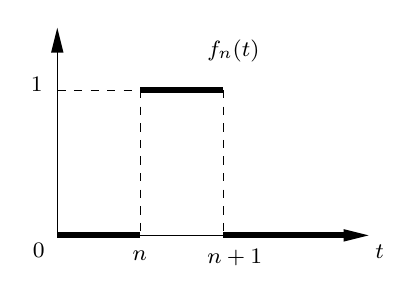
\begin{tikzpicture}[x=0.75pt,y=0.75pt,yscale=-1,xscale=1]
	%uncomment if require: \path (0,257); %set diagram left start at 0, and has height of 257

	\draw    (220,170) -- (368,170) ;
	\draw [shift={(370,170)}, rotate = 180] [fill={rgb, 255:red, 0; green, 0; blue, 0 }  ][line width=0.08]  [draw opacity=0] (12,-3) -- (0,0) -- (12,3) -- cycle    ;
	\draw    (220,170) -- (220,72) ;
	\draw [shift={(220,70)}, rotate = 90] [fill={rgb, 255:red, 0; green, 0; blue, 0 }  ][line width=0.08]  [draw opacity=0] (12,-3) -- (0,0) -- (12,3) -- cycle    ;
	\draw  [dashed, very thin]  (260,100) -- (260,170) ;
	\draw [line width=2.25]    (260,100) -- (300,100) ;
	\draw  [dashed, very thin]  (300,100) -- (300,170) ;
	\draw [line width=2.25]    (220,170) -- (260,170) ;
	\draw [line width=2.25]    (300,170) -- (360,170) ;
	\draw  [dashed, very thin]  (220,100) -- (260,100) ;

	\draw (207,172.4) node [anchor=north west][inner sep=0.75pt]  [font=\footnotesize]  {$0$};
	\draw (372,173.4) node [anchor=north west][inner sep=0.75pt]  [font=\footnotesize]  {$t$};
	\draw (206,92.4) node [anchor=north west][inner sep=0.75pt]  [font=\footnotesize]  {$1$};
	\draw (291,74.4) node [anchor=north west][inner sep=0.75pt]  [font=\footnotesize]  {$f_{n}( t)$};
	\draw (255,176.4) node [anchor=north west][inner sep=0.75pt]  [font=\footnotesize]  {$n$};
	\draw (291,175.4) node [anchor=north west][inner sep=0.75pt]  [font=\footnotesize]  {$n+1$};
	\end{tikzpicture}
\end{figure}
\FloatBarrier
See that $f_n \aeto 0$. However, there exist $\eps>0$ and $E\subset\RR$ such that $\lambda(E)<\eps$ and:
	$$\sup_{\RR \setminus E} |f_n| = 1 \not\to 0  \text{ as } n \to +\infty.$$

\paragraph{Point-wise a.e.\ convergence does NOT imply convergence in mean} Consider the following counterexample.

Take $\Omega = [0, 1]$ and:
$$f_n(t)=\begin{cases}
	n^2 & \text{if } 0\leq t < \frac 1 n \\
	0 & \text{if } \frac 1 n \leq t \leq 1.\\
	\end{cases}$$
Then $f_n$ converges a.e. to $0$, but $\int_{0}^{1} f_n \,\dlam = n$ and its limit is $+\infty$, thus $f_n$ does not converges in mean to $0$.

Also this implication can be restored if we add more strict hypotheses. If a series of functions respects the requirements of the dominated convergence theorem (see \vref{dominated-convergence}) then, if the series converges point-wisely a.e. we have that it converges in mean as well.

\paragraph{Uniform a.e.\ convergence does NOT imply convergence in mean} This can be deduced from the previous results, otherwise it would be a contradiction.

For a counterexample consider the series function $f_n = \tfrac 1 n \Ind_{(0,n)}(t)$, with $n \in \NN_0$.\\
Then $f_n$ converges a.e. to $0$, but $\int_{0}^{+\infty}f_n \, \dlam = 1$ for all $n\in \NN_0$.
Since uniform a.e. convergence implies point-wise a.e. convergence and, with the hypothesis of dominated convergence, it implies the convergence in mean, this convergence can be restored if the hypothesis of that theorem are fulfilled.

\paragraph{Convergence in mean does NOT imply point-wise a.e.\ convergence} In this case, consider the counterexample of the \textit{typewriter sequence}.

Take $\Omega = [0, 1]$ and $\mu = \lambda$, the Lebesgue's measure. For $k \in \NN$ consider $m \in \{0,1,2,\ldots,2^k-1\}$, calculate $n = 2^k + m$ and define:
$$E_n = \left[\frac m {2^k},\frac {m+1}{2^k}\right].$$
We have, for each $k$, a partition of $[0,1]$, where $E_n$ fill the interval from left to right as a typewriter moves each line down and from left to right in each line.
For instance we have the following sets:
\begin{align*}
	k=0 \qquad &  m \in \{0\} \qquad & n = 1 \qquad &  E_1= \left[0, 1\right]\\
	k=1 \qquad &  m \in \{0,1\} \qquad & n = 2 \qquad &  E_2= \left[0, \frac 1 2\right]\\
	& & n = 3 \qquad &  E_3= \left[\frac 1 2, 1\right]\\
	k=2 \qquad &  m \in \{0,1,2,3\} \qquad & n = 4 \qquad &  E_4= \left[0, \frac 1 4\right]\\
	& & n = 5 \qquad &  E_5= \left[\frac 1 4,\frac 1 2\right]\\
	& & n = 6 \qquad &  E_6= \left[\frac 1 2, \frac 3 4\right]\\
	& & n = 7 \qquad &  E_7= \left[\frac 3 4, 1\right]\\
	k=3 \qquad &  m \in \{0,1,2,3,4,5,6,7\} \qquad & n = 8 \qquad &  E_8= \left[0, \frac 1 8\right]\\
\end{align*}
$$\cdots$$
	
Take $f_n = \Ind_{E_n}$, as in figure \vref{fig:typewriter}.
% https://math.stackexchange.com/questions/1412091/the-typewriter-sequence/2894204
\begin{figure}[htpb]
	\centering
	\newcommand{\nMAX}{15} 
	\begin{tikzpicture}[font=\Large,shorten >=-2.5pt,shorten <=-2.5pt,yscale=0.3,xscale=0.3]
	\begin{axis}[
	    axis x line*=bottom,
	    axis y line*=right,
	    axis z line*=left,  
	    plot box ratio = 3 1000 2,
	    view={.3}{.2},  
	    xmin=-0.2,    xmax=1.25,         
	    ymin=0.6,    ymax=\nMAX+0.3,                                 
	    zmin=0,    zmax=1.0,
	    xtick={0,1/8,2/8,3/8,4/8,5/8,6/8,7/8,1},
	    xticklabels={$0$,$\frac{1}{2^3}$,$\frac{2}{2^3}$,$\frac{3}{2^3}$,$\frac{4}{2^3}$,$\frac{5}{2^3}$,$\frac{6}{2^3}$,$\frac{7}{2^3}$,$1$},
	    ytick={0,...,\nMAX},    
	    ztick={0,...,1.0},       
	    xlabel=$x$,
	    ylabel=$n$,
	    zlabel=$f_n(x)$,
	    x label style={at={(axis description cs:0.067,-0.001)},anchor=north},
	    y label style={at={(axis description cs:0.062,0.145)},anchor=south},    
	    z label style={at={(axis description cs:-0.002,0.035)},anchor=south},     
	    yscale=5,
	    xscale=5,
	    legend entries={$f_n(x)=1\,$,
	                    $f_n(x)=0\,$},
	    legend style={at={(0.023,0.14)}},   
	    legend style={nodes={scale=1.5, transform shape}},
	    legend plot pos=right,
	]
	\foreach \n in {1, ..., \nMAX} 
	{
	    \pgfmathsetmacro\k{floor(log2(\n+1e-1))}
	    \pgfmathsetmacro{\xm}{-0.2}
	    \pgfmathsetmacro\xM{1.2}
	    \pgfmathsetmacro\xa{(\n-(2^(\k)))/(2^(\k))}
	    \pgfmathsetmacro\xb{(\n-(2^(\k))+1)/(2^(\k))}
	    \edef\temp
	    {
	        \noexpand\coordinate (d1) at (axis cs:\xm,\n,0);
	        \noexpand\coordinate (d2) at (axis cs:\xa,\n,0);    
	        \noexpand\coordinate (d3) at (axis cs:\xa,\n,1);
	        \noexpand\coordinate (d4) at (axis cs:\xb,\n,1);    
	        \noexpand\coordinate (d5) at (axis cs:\xb,\n,0);        
	        \noexpand\coordinate (d6) at (axis cs:\xM,\n,0);    
	        \noexpand\coordinate (g0) at (axis cs:\xm,\n,1);
	        \noexpand\coordinate (g1) at (axis cs:\xM,\n,1);                
	    }
	    \temp
	    \draw[blue,dashdotted,thick,<-o] (d1)--(d2);
	    \draw[black,dashed,line width=0.04mm,opacity=0.5] (d2)--(d3);
	    \draw[black,dashed,line width=0.04mm,opacity=0.5] (d4)--(d5);       
	    \draw[blue,dashdotted,thick,o->] (d5)--(d6); 
	    \draw[black,dashed,line width=0.04mm,opacity=0.5] (g0)--(g1);
	    \draw[very thick,red,*-*]   (d3)--(d4);   
	}
	\pgfplotsinvokeforeach{0, ..., 8} 
	{
	    \draw[black,dashed,line width=0.06mm,opacity=0.5] (axis cs:#1/8,0,0)--(axis cs:#1/8,\nMAX,0);
	}   
	\addlegendimage{no markers,very thick,red}
	\addlegendimage{no markers,blue,dashdotted,thick}
	\end{axis}
	\end{tikzpicture}
	\caption{The typewriter sequence.}
	\label{fig:typewriter}
\end{figure}

Then
$$\int_0^1 \Ind_{E_n} \,\dlam =
\frac 1 {2^k} = \frac 1 {n-m}
\to 0
\text{ as } n \to +\infty$$
and thus $f_n$ converges in mean to $0$.\\
However, $\lim_{n\to \infty} \Ind_{E_n}(t)$ does not exist for any $t \in \left[0,1\right]$, and thus $f_n$ does not converge point-wise to any function.


We have the following proposition, as we can restore the implication for only a subsequence.
\begin{prop}\label{convergence-mean-implie-subsequence-ae}
	If $f_n \lto{1} f$, then there exists a sub-sequence $\{f_{n_h}\}$ such that $f_{n_h} \aeto f$.
\end{prop}
This is a trivial corollary of the proposition \vref{convergence-mean-implies-convergence-measure} that we will see.	

\paragraph{Convergence in mean does NOT imply uniform a.e.\ convergence} Otherwise we would have a contradiction. To restore the convergence, some additional hypothesis are required.

\paragraph{Convergence in measure does NOT imply point-wise a.e.\ convergence} The counterexample of the \textit{typewriter sequence} fits again.
We know that $\Ind_{E_n}$ does not converge point-wisely to any $f$, but it is easy to check that $\Ind_{E_n} \mto 0$. Indeed:
$$\lambda (\{t\in \left[0,1\right]:\Ind_{E_n}(t) > \delta\} < \frac {1}{2^k}
\quad \forall \delta > 0.$$

Nonetheless, the following result holds.
\begin{prop}\label{convergence-measure-implie-subsequence-ae}
	If $f_n \mto f$, then there exists a sub-sequence $\{f_{n_h}\}$ such that $f_{n_h} \aeto f$.
\end{prop}

\begin{proof}
	Let $\delta_n >0$ such that $\delta_n \to 0$, and $\eps_n > 0$ be such that $\sum_{n\in \NN} \eps_n < +\infty$.\\
	Consider a sub-sequence $\{n_h\}$, with $n_h>n_{h-1}$, such that:
	$$ E_h = \{t \in \Omega:|f_{n_h}(t)-f(t)|>\delta_{n_h}\} \text{ and } \mu(E_h) < \varepsilon_{n_h} . $$
	Set $E=\bigcap_{h\in \NN}E_h$.\\
	Since $\mu(E_h)\leq\sum_{h\in \NN}\eps_{n_h} < +\infty$ and $\{E_h\}$ is monotone decreasing, we have that $\mu(E_h) \downarrow \mu(E)$. \\
	Moreover, $\mu(E_h) \leq \sum_{j=n}^{\infty} \eps_{n_j} \to 0$ as $h \to \infty$, and thus $\mu(E)=0$.
	
	Take now $t\in E\comp$. Then $\exists \, k \in \NN$ such that $t\notin E_k$, that is, $|f_{n_k}(t)-f(t)| \leq \delta_{n_k}$. \\
	Thus $f_{n_h}(t) \to f(t) \enspace \forall h \geq k \enspace \forall t \in E\comp$.
\end{proof}

\paragraph{Point-wise a.e.\ convergence does NOT imply convergence in measure} Nevertheless, we have the following result.

\begin{prop}\label{convergence-point-wise-omega-finite-imply-measure}
	If a series of function converges point-wisely almost everywhere, then such series also converges in measure if $\mu(\Omega) < +\infty$.
\end{prop}
\begin{proof}
	Let $E \in \mm$ such that $\mu(E)=0$ and:
	$$f_n(t) \not\to f(t) \text{ if } t\in E, \quad f_n(t) \to f(t) \text{ if } t\in E\comp.$$
	
	Fix $\delta > 0$ and consider:
	$$A_k(\delta) = \{t \in \RR:|f_k(t)-f(t)| > \delta\}, \quad
	B_n (\delta) = \bigcup_{k=n}^\infty A_k(\delta), \quad
	C(\delta) = \bigcap_{n\in \NN} B_n(\delta).$$
	
	See that $B_n$ is decreasing, namely $B_1 \supset B_2 \supset \cdots \supset B_n$, and $\mu(B_1)<+\infty$.\\
	Then $\mu(B_n(\delta)) \to \mu(C(\delta))$.
	
	Notice that $C(\delta) \subset E$. Indeed:
	\begin{align*}
	t \in C(\delta)
	&\implies f \in B_n(\delta) \ \forall n \in \NN \\
	&\implies \forall n \ \exists \, k \geq n : t\in A_k \\
	&\implies \forall n \ \exists \, k \geq n : |f_k(t)-f(t)|>\delta \\
	&\implies f_n(t) \not\to f(t)
	\implies t \in E
	\end{align*}
	Then $\mu (C(\delta))=0$, and thus $\mu(B_n (\delta)) \to 0$. \\
	However $A_n(\delta) \subset B_n(\delta)$, thus also $\mu (A_n(\delta)) \to 0$ as $n\to \infty$, that is $f_n \mto f$.
\end{proof}

If the hypothesis is not satisfied the thesis is not guaranteed, indeed consider for example that $\mu(\Omega) = +\infty$ and set:
$$f_n(t) = \begin{cases}
1 & \text{if } t\geq n \\
0 & \text{if } t<n
\end{cases} \quad \forall n \in \NN.$$
Then $f_n \aeto 0$, but $\lambda (\{t \in \RR : f_n(t) > \frac 1 2\}) = +\infty$ $\forall n \in \NN$, and thus  $f_n \xslashedrightarrow{\lambda} 0$. Notice that if $\{f_n\}$ would converge in measure then it would necessarily converge to $0$.

\paragraph{Convergence in mean implies convergence in measure} For this last case, the following result holds.
\begin{prop}\label{convergence-mean-implies-convergence-measure}
	If a series of function converges in mean, then such series also converges in measure.
\end{prop}
\begin{proof}
	Fix $\delta > 0$, and set $E(\delta) \coloneqq \{t\in \Omega: |f_n(t)-f(t)| > \delta\}$. We want to prove that $\mu(\delta) \to 0$ as $n \to +\infty$. We have, by monotonicity:
	$$\int_\Omega |f_n-f| \,\de\mu
	\geq \int_{E(\delta)} |f_n-f| \,\de\mu
	\geq \delta\mu(E).$$
	Since $\int_\Omega |f_n-f| \,\de\mu \to 0$ as $n \to +\infty$, then also $\delta \mu(E) \to 0$.
\end{proof}

But the inverse is not true, as shown here.

\paragraph{Convergence in measure does NOT imply convergence in mean} indeed, consider the measure space $(\RR,\Lc(\RR), \lambda)$ and take $f_n(t) \coloneqq n \Ind_{\left[0,\frac 1 n\right]}(t)$.\\
Then $\lambda(\{t \in \RR : f_n(t) > \delta \}) \leq \frac 1 n \to 0$ as $n\to \infty$, and thus $f_n \mto 0$.\\
However $\int_0^1 f_n(t) \,\dlam=1$ as $n\to \infty$, and thus $f_n \xslashedrightarrow{\mu} 0$.



\paragraph{Summary of the relations between kinds of convergence} we stated the following relations between convergences: 

\begin{enumerate}
	\item \emph{uniform a.e.\ convergence implies point-wise a.e.\ convergence}, see theorem \vref{convergence-uniform-implies-point-wise}, whose proof is left to the reader;
	\item \emph{point-wise a.e.\ convergence does NOT imply uniform a.e.\ convergence}, as shown with a counterexample, but the implication can be restored as specified in Severini--Egorov theorem (\vref{prop-sever-egoro});
	\item \emph{point-wise a.e.\ convergence does NOT imply convergence in mean}, as shown with a counterexample, but the implication can be restored if the hypothesis of dominated convergence theorem (\vref{dominated-convergence}) are fulfilled;
	\item \emph{uniform a.e.\ convergence does NOT imply convergence in mean}, as shown with a counterexample, but the implication can be restored if the hypothesis of dominated convergence theorem (\vref{dominated-convergence}) are fulfilled;
	\item \emph{convergence in mean does NOT imply point-wise a.e.\ convergence}, as shown with the typewriter counterexample, but the implication can be restored for a sub-sequence, see proposition \vref{convergence-measure-implie-subsequence-ae};
	\item \emph{convergence in mean does NOT imply uniform a.e.\ convergence} otherwise we would have a contradiction, but the implication can be restored with the tools introduced for the previous cases;
	\item \emph{convergence in measure does NOT imply point-wise a.e.\ convergence}, as shown with the typewriter counterexample, but the implication can be restored for a sub-sequence, see proposition \vref{convergence-mean-implie-subsequence-ae};
	\item \emph{point-wise a.e.\ convergence does NOT imply convergence in measure}, unless the domain has finite measure, see proposition \vref{convergence-point-wise-omega-finite-imply-measure};
	\item \emph{convergence in mean implies convergence in measure}, see theorem \vref{convergence-mean-implies-convergence-measure};
	\item \emph{convergence in measure does NOT imply convergence in mean}, as shown with a counterexample.
\end{enumerate}


\begin{figure}[htpb]
	\centering
	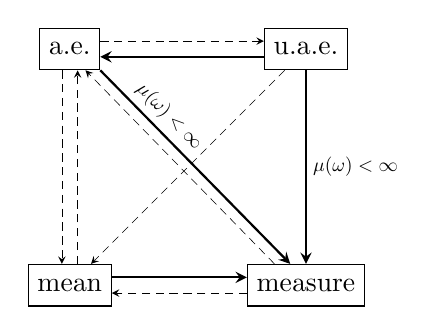
\begin{tikzpicture}
		\tikzset{
		    vertex/.style={rectangle,draw,minimum size=1.5em},
		    edge/.style={->,> = stealth, thick},
		    notimplies/.style={edge,densely dashed, very thin}
		}

		% vertices
		\node[vertex] (ae) at (0,3) {a.e.};
		\node[vertex] (uae) at (3,3) {u.a.e.};
		\node[vertex] (mean) at (0,0) {mean};
		\node[vertex] (measure) at (3,0) {measure};

		%edges
		\draw[edge] ([shift=({0,-0.1})]uae.west) -- ([shift=({0,-0.1})]ae.east) {};
		\draw[edge] ([shift=({0,0.1})]mean.east) -- ([shift=({0,0.1})]measure.west) {};
		\draw[edge] (ae.south east) -- ([shift=({-0.2,0})]measure.north) node[midway,above,sloped,rotate=0,scale=.7,pos=0.3] {$\mu(\omega)<\infty$};
		\draw[edge] (uae) -- (measure) node[midway,right,sloped,rotate=90,scale=.7] {$\mu(\omega)<\infty$};

		\draw[notimplies] ([shift=({0,0.1})]ae.east) -- ([shift=({0,0.1})]uae.west) {};
		\draw[notimplies] (uae) -- (mean) {};
		\draw[notimplies] ([shift=({0.1,0})]mean.north) -- ([shift=({0.1,0})]ae.south) {};
		\draw[notimplies] ([shift=({-0.1,0})]ae.south) -- ([shift=({-0.1,0})]mean.north) {};
		\draw[notimplies] ([shift=({0,-0.1})]measure.west) -- ([shift=({0,-0.1})]mean.east) {};
		\draw[notimplies] ([shift=({-0.4,0})]measure.north) -- ([shift=({0.2,0})]ae.south) {};

	\end{tikzpicture}
	\caption{Summary of the implication of convergences. Solid: implied (potentially under some condition specified along the line); dashed: not implied.}
\end{figure}
\FloatBarrier

To conclude our discussion we present the following result about convergence in measure.
\begin{prop}
	If $f_n\mto f$ and $f_n \mto g$, then $f=g$ a.e.
\end{prop}

The space $L^1$ belongs to the family of functional space called ``$L^p$ spaces''. In particular the distance $d_\infty(f,g) = \esssup |f - g|$ is a metric related to the space $L^\infty$, as $(L^\infty, d_\infty)$ is a metric space. A wider discussion occurs in section \vref{chapter-Lp-spaces}.

%\paragraph{The space $L^\infty$}
%
%The space $\Lc^\infty$ is the set of measurable functions that bounded a.e., namely:
%$$\Lc_\infty(\Omega, \mm, \mu) = \{f_\Omega \to \RR \text{ such that } f \text{ is measurable and essentially bounded}\}.$$
%As we have done for $\Lc^1$ we quotient set with respect to the equivalence relation $f\sim g$ if $f=g$ a.e..
%$$L_\infty(\Omega, \mm, \mu)=\frac{\Lc_\infty(\Omega, \mm, \mu)}{\sim}.$$
%
%Such set is a vector space on $\RR$ with respect to the canonical operations sum $[f]+[g]=[f+g]$ and scalar multiplication $[c f] = c[f]$, $c \in \RR$. It is also a metric space with respect to the distance $$d_\infty = \esssup_\Omega |f-g| \quad [f],[g]\in L_\infty(\Omega, \mm, \mu).$$

\paragraph{Metric convergence} 
Some convergence can be induced by a metric, in such case they are said to be \emph{metric convergences}.\\
The \textit{uniform a.e.\ convergence} is induced by the $d_\infty$ metric; indeed, we have:
$$
	d_\infty(f_n,f) 
	\to 0 
	\iff f_n 
	\uaeto f
.
$$

The \textit{convergence in mean} is a metric convergence too, as it is inducted by $d_1$:
$$
	d_1(f_n,f) 
	\to 0 
	\iff f_n 
	\lto{1} f
.
$$

The \textit{point-wise a.e.\ convergence} is not induced by any metric, so it is not a metric convergence. Some exceptions could occur, in particular when the measure $\mu$ is positive only on a countable set.

The case of \textit{measure convergence} is a bit more complicated. We have to operate on a proper space and define a proper metric.\\
Consider the measure space $(\Omega, \mm, \mu)$ where $\mu$ is finite, and the following space:
$$
	\Fc 
	\coloneqq \{f:\Omega \to \RR \text{ measurable}\}
;
$$
then consider related quotient space $\Uc \coloneqq \frac{\Fc}{\sim}$ defined with the following equivalence relation:
$$
	f
	\sim g 
	\iff 
	f
	=g 
	\quad \text{a.e.}
,
$$
that includes all the functions which are equal a.e.\ to a measurable one.
Now define the following distance:
$$
	d_\mu(f,g) 
	\coloneqq \int_\Omega \frac{|f-g|}{1+|f-g|} \; \de\mu
.$$
This is a metric in $\Uc$ and $(\Uc, d_\mu)$ is a complete metric space.\\
The measure convergence is a metric convergence with the distance $d_\mu$, namely:
$$
	d_\mu(f_n,f) 
	\to 0 
	\iff 
	f_n 
	\mto f 
	\quad \text{as } n \to +\infty
.
$$

%Uniform a.e. convergence and mean convergence are metric convergences:
%$$
%d_\infty(f_n,f) 
%\to 0 
%\iff f_n 
%\uaeto f \text{ and } d_\infty(f_n,f) \to 0 \iff f_n \lto{1} f.$$
%The point-wise a.e. convergence is not induce by any metric, while convergence in measure can be induced by a metric if $\mu(\Omega) < \infty$, and we have:
%$$\rho(f_n,f) = \int_\Omega \frac{|f_n-f|}{1+|f_n-f|} \, \de\mu \iff f_n \mto f.$$
%
%\begin{prop}
%	Consider the measure space $(\Omega, \mm, \mu)$ where $\mu$ is finite, and the following space:
%	$$\Fc \coloneqq \{f:\Omega \to \RR \text{ measurable}\}$$
%	Consider also the related quotient space $\Uc \coloneqq \frac{\Fc}{\sim}$ with the following equivalence relation:
%	$$f\sim g \iff f=g \quad \mu\text{-a.e.}$$
%	Let now:
%	$$d_\mu(f,g) \coloneqq \int_\Omega \frac{|f-g|}{1+|f-g|} \de\mu$$
%	Then $d_\mu$ is a metric in $\Uc$, $(\Uc, d_\mu)$ is a complete metric space\todo{Which $\sigma$-algebra?}, and we have:
%	$$d_\mu(f_n,f) \to 0 \iff f_n \mto f \quad \text{as } n \to +\infty$$
%\end{prop}
%The proof of the two previous results is left as an exercise for the reader.

%\begin{prop}
%	Consider the measure space of essentially bounded measurable functions $B(\Omega,\mm,\mu)$. Let:
%	$$d_B(f,g)\coloneqq\esssup_{\Omega}|f-g|$$
%	Then $d_B$ is a metric and we have:
%	$$d_B(f_n,f) \to 0 \iff f_n \uaeto f \quad \text{as } n \to +\infty$$
%\end{prop}
%
%In general, point-wise convergence is not associate with a metric, with the exception of very special cases (\textit{e.g.} $\mu$ is concentrated on a countable set).


%!!!!! once upon a time, here there was the Radon--Nikodym Derivative
